% !TEX root = ../thesis.tex
\chapter{Utilized Tools}
\label{chap:Utilized Tools}


\section{Openstack}
\label{sec:openstack}
\subsection{overview}
OpenStack is a free and open-source software consisting in a series of interrelated projects that control pools of processing, storage, and networking resources throughout a data-center.
This project, started in 2010, aims to behave as a data-center operating system or cloud OS.
As a classical one, a cloud operating system's main purpose is to export an abstraction of the controlled physical hardware but, instead of piloting directly the integrated circuits via drivers as in the single server case, it has the ability to interface itself with an arbitrary number of agents resident over the hypervisor operating system of each physical server, in other words it behaves as an hypervisor of hypervisors.
The OpenStack project aims to provide a centralized interface to be used by data-center administrators, giving them an overview about resources  availability, usage and status and therefore putting them in the position to plan maintenance or provision hardware resizing in order to keep up with the demanded computational power.
Being a commercial product and not only a proof of concept, OpenStack is also engineered to permit the coexistence of administrators and normal users, the firsts are in charge of monitoring the resources availability and manage the infrastructure of the data-center providing the seconds the possibility to instantiate virtual machines and interconnecting them without worrying about configuring the physical infrastructure and actually available resources.
Normal user is a general term that will refer to a person that does not have administrative privileges (e.g. does not have full control over the system), in the case of this software, a user can correspond to either a single person, a department in a company or even to an entire firm that decides to rely on an external infrastructure in where to deploy the virtual servers that provide the services needed to run its business.
The usage of a cloud operating system is highly recommended even for a private data-center (e.g. used only by the company who owns it), the reasons are numerous, for example management simplicity, resources consolidation and users isolation.
Of course this automation and level of abstraction come at a price which is affordable without any problem in a data-center environment, on the other hand in the case of very small amount of physical machines the overhead is not negligible even if not exaggerate.
Let's say that in general, when the number of equipment exceed the few units and the virtual machines creation and deletion volume is high enough to overload the amount of requests that administrators can keep up with, the effort to install the OpenStack system will be well rewarded.

\subsection{General design architecture}
OpenStack has been developed with five guidelines which are:
\begin{itemize}
    \item Component based architecture, to quickly add new behaviors.
    \item Highly capable of easily scale up/down.
    \item Fault tolerant, isolated processes avoid cascading failures.
    \item Recoverable, failures should be easy to diagnose, debug, and rectify.
    \item Open standards, be a reference implementation for a community-driven API.
\end{itemize}
As said before and enhanced by the first design principle, OpenStack is not a single project but a pool of independent modules that communicate together, each one in charge of providing one or more functionalities (e.g. computing and network management, authentication, etc).
Modularity has two main benefits, the first one is to permit data-center administrators to choose what features they want and what they don't, enabling the possibility to offer users different typologies of service; the second advantage is the interchangeability of modules designed for the same purpose (e.g. network management) so that an administrator can pick the one module that suits the best or even write one by himself/herself from scratch.
The majority of modules are, in turn, splitted into submodules and projected to allow plugging in special purpose add-ons written to accomplish specific tasks or made the module behave in a certain desired way.
\subsection{Physical architecture}
The deployment of OpenStack requires a total amount of three logically separated entities which can be remapped into one or more baremetal machines.
These three entities are generally referred as the following:
\begin{itemize}
    \item Controller node.
    \item Compute node.
    \item Network node.
\end{itemize}

In the controller node resides a set of supporting services, basic (or core) components and a series of optional features.
Supporting services are not properly OpenStack components but are necessary for its operations such as a database management system and a message broker. Having them in the controller node is not mandatory but since the major share of requests to this components comes from services also resident in the control node, delays due to the network are eliminated.
For basic services are intended all those OpenStack components that provide the very basic functionalities and that will become the "brain" in charge of managing the whole infrastructure.
In addition in the controller node can be installed optional components that are not crucial but offers useful functionalities such as a telemetry service - Ceilometer - that will track resources usage aggregated by user and comes very handy to manage the billing in case of a data-center offered as a service or in the case of the orchestration component known as Heat that is in charge of communicating both with the networking and the compute manager. The controller node needs to communicate directly with all the other nodes (management interface) to dispatch commands and receive updates from all the deployed agents.

The compute node is in charge of actually hosting the virtual machines. This node is associable to a single physical server while the controller node is the brain of OpenStack, this kind of node is the muscles, will be the identity that each hardware machine will assume. Since all the control services are hosted in the controller node, the amount of software required to be installed in this kind of node is minimal saving computing resources for the virtual instances that will be deployed. The only pieces of code required are an agent that communicates with the local hypervisor and - optionally - one that takes care of accepting particular commands to provide traffic isolation between users. In addition to that, in the case of usage of optional services that requires a distributed agent to retrieve statistics, also these agents are obviously required.
Compute nodes are connected to the controller node to receive instructions and have a logically separated "instance tunnel" interface to communicate with each other in order to permit users' VMs to exchange traffic. An edge of this network is the Network node.

The Network node is the border between the OpenStack and the outside world, in particular is in charge of being the only node that has the capability to connect to the external network and let VMs traffic in and out to the Internet. It is also connected to the Controller node to receive commands. In this frontier component are instantiated not VMs but agents that will be in charge of providing basilar network services such as network address translation (NAT), ip assignation (DHCP) and privacy policies via a firewall.

\label{a:br_section}
In the classical architecture, each compute node have two virtual switches that can either be linux bridges, openvswitches\cite{ovswebsite} or xDPd\cite{xdpdwebsite}, one for attaching the VMs (generally called br-int) and the other (referred as br-net or br-tun) to create virtual tunnels with the other compute nodes establishing a full mesh network that will carry packets from one server to another making the intermediate network infrastructure completely transparent. Also the network node has these two virtual bridge instances and in addition has another one (usually known as br-ex). To this software switch is bridged the physical network interface card (NIC) that has access to the Internet.
The br-int and the br-ex in the network node are not linked in any way so that traffic cannot exit the inside of the data-center nor outside packets can enter the private network unless a specific service (a router) is deployed and linked with two virtual interfaces, one connected to each software switch.

A logical schema for better understanding the complex architecture is provided in figure  \ref{fig:OSarchitecture}, more details of the depicted services are available in section \ref{a:main_components}.
\begin{figure}[h]
	\centering
	% left bottom right top
	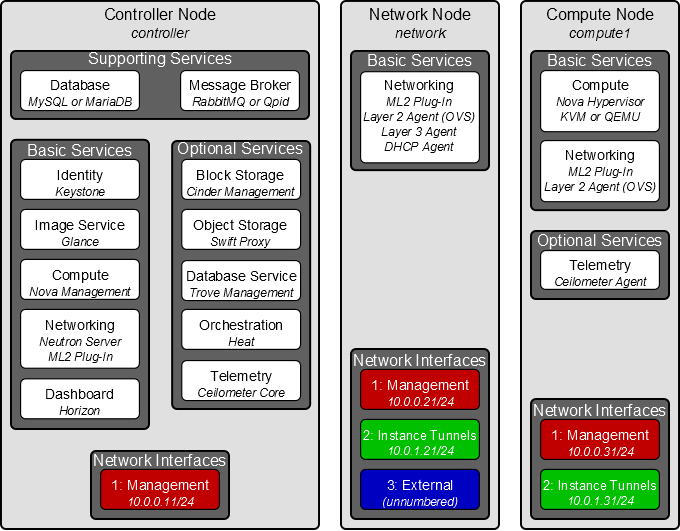
\includegraphics[clip= true, width= \columnwidth]{images/openstack_nodes.png}
	\caption{OpenStack logical nodes - services and interfaces}
	\label{fig:OSarchitecture}
\end{figure}

%aggregation of logical entities
The above described logical architecture, depending on the size and computing power of the data-center, can be remapped in various way, in particular the three entities can be aggregated as the administrator is likes at installation time, a common deployment is to devolve one server serving as controller node and one as a network node, plus as many as pleased behaving as compute nodes. Even if the most adopted, the one described is not the only solution, in case of a very small data-center in which there are just some physical machines nodes can be collapsed. As the opposite bound to the above scenario, OpenStack can be used to manage just one server; in this particular case one single machine will have all the three entities at the same time. Evidently the last example is a critical situation in which the introduced overhead is really influencing the performances, therefore this kind of configuration is useful only for developing and testing purposes.

\begin{table}[h]
\matteo{insert data}
\label{tbl:resource_usage}
\centering
\begin{tabular}{c|c|c|c|}
\cline{2-4}
\textbf{}                                                             & \textbf{CPU}       & \textbf{RAM}       & \textbf{DISK}   \\ \hline
\multicolumn{1}{|l|}{\textbf{controller node - full installation}}    & \textbf{XXX GB}    & \textbf{2.1 GB}    & \textbf{XXX GB} \\ \hline
\multicolumn{1}{|l|}{\textbf{controller node - minimal installation}} & \textbf{XXX GB}    & \textbf{1.5 GB}    & \textbf{XXX GB} \\ \hline
\multicolumn{1}{|l|}{\textbf{compute node}}                           & \textbf{XXX GB}    & \textbf{590 MB}    & \textbf{XXX GB} \\ \hline
\multicolumn{1}{|l|}{\textbf{network node}}                           & \textbf{XXX GB}    & \textbf{250 MB}    & \textbf{XXX GB} \\ \hline
\end{tabular}
\caption{OpenStack nodes - resource analysis}
\end{table}

\subsection{Main components}
\label{a:main_components}
OpenStack modules (from now on called services) communicates together either via RESTful API or via a messaging server and may have the need to query a database. Additionally, in case of a data-center as a service provided to external users, it offers a web interface - the Horizon dashboard - that requires a web server in order to serve users' requests.
These three additional services are not part of the core components of OpenStack but, based on the standard configuration, they are necessary and essential for the system to work properly.
As visible in figure \ref{fig:OS_components_interraction_logical} where the main components and their interactions are represented, the services are clearly separated by functionality. Also looking at the image is evident that two components are more involved in communications compared to the others. These two components are the previously cited dashboard that as said is optional but highly recommended and the identity service that provides authentication to both services and users.
\begin{figure}[h]
	\centering
	% left bottom right top
	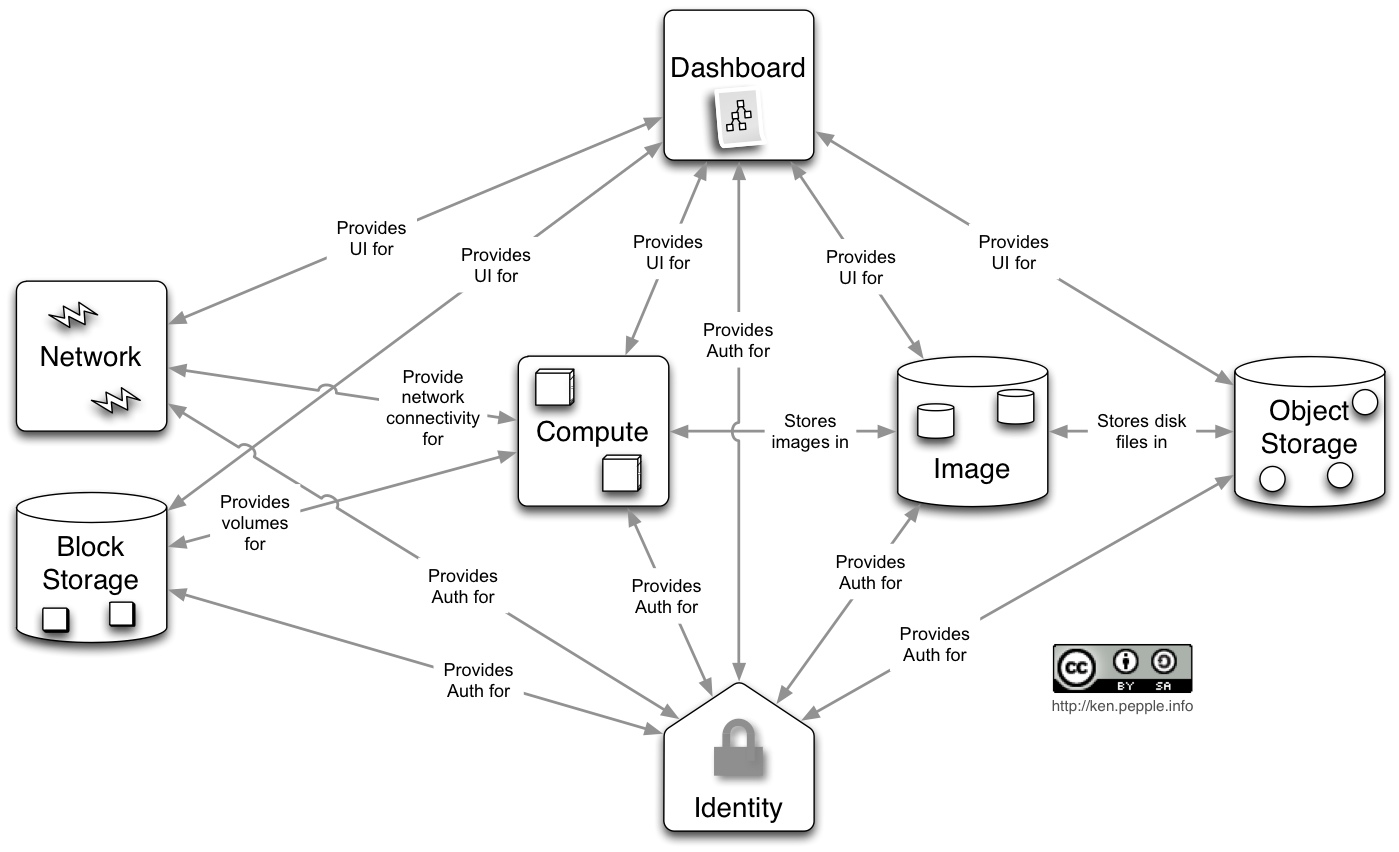
\includegraphics[clip= true, width= \columnwidth]{images/openstack_core_components.jpg}
	\caption{OpenStack - components interaction}
	\label{fig:OS_components_interraction_logical}
\end{figure}
\subsubsection{Identity - keystone}
\label{sec:keystone}
Keystone:




As a distributed environment, the system has to provide secure access and in order to achieve that both users and services must authenticate themselves before performing any operation.

OpenStack developers wrote a specific service called keystone for this vary purpose, in it are stored username and password for each authorized user/service, the authorization process involves obtaining a token to be used later to perform requests to other services. The general concept behind a token-based authentication system is simple. Allow users to enter their username and password in order to obtain a token which allows them to fetch a specific resource - without using their username and password. Once their token has been obtained, the user can offer the token - which offers access to a specific resource for a time period. Identity also correlate to a user its role in the system and the visibility of resources he or she can get. Administrators are able to see everything that is going on in the system while a common user can only see the virtual resources he or she created.

This separation of group belonging, or to better say membership, in keystone is called role and is used by other services to check whether the user is authorized or not to perform such operation, basically defining a sandbox for each user so that anyone can only see what he or she is authorized to.

Alongside the user concept, keystone defines three fundamental terms which are group, tenant (or project) and domain; in this way rules can be associated to them instead of directly to a user. These terms are remapped to internal data-types, here below a list of keystone objects is given alongside with a brief description and usage:

\begin{itemize}

\item User: has account credentials, is associated with one or more projects or domains.

\item Group: a collection of users, is associated with one or more projects or domains.

\item Project: unit of ownership in OpenStack, contains one or more users. Project and tenant terms are used indiscriminately because of historical reasons since the name has changed throughout the course of releases.

\item Domain: contains users, groups and projects.

\item Role: a first-class piece of metadata associated with many user-project pairs.

\item Token: identify credential related to a user or to a user-project pair.

\item Extras: bucket of key-value metadata associated with a user-project pair; its main usage is intended to provide a method to send extra fields in a REST call without changing its interface.

\item Rule: describes a set of requirements for performing an action.

\end{itemize}

Since credentials are generally built from the user metadata in the \texttt{"extras"} field of the Identity API, adding a \texttt{"role"} to a user just means to add the role to the metadata.

Data types are used inside keystone to provide a set of services that are exposed to users via one or more endpoints:

\begin{itemize}

\item Identity - this service is intended to provide authentication, credential validation and data about Users, Groups, Projects, Domains and Roles, as well as any associated metadata. In the basic case all these data is managed directly by the service itself that exposes all the CRUD methods associated with the data. In other cases this data is pulled, by varying degrees, from an authoritative backend service such as LDAP. 

\item Token - The token service validates and manages tokens that are used when performing requests, typically to other services; a token is created once a user credentials have been verified.

\item Catalog - The catalog service provides a registry used for endpoint discovery, this permits to know how to contact all the other services.

\item Policy - this last but not least service provides a rule-based authorization engine and the associated rule management interface.

\end{itemize}

Policies based on a set of rules can be specified for each OpenStack component; all components have their own \texttt{"policy.json"} file that permits to associate rules to all Openstack service actions. The following is an example of policy.json file of Compute service (Nova) in which is defined - lines 14 and 15 - a policy that only permits to the user identified as the owner or an administrator to start or stop a VM, meaning that someone that shares a project with the previous user is not allowed to manage a VM not belonging to him/her.

\lstinputlisting[label=lst:nova_policy, language=python, caption={policy.json file relative to the Nova service}]{code/nova_policy.json}





\subsubsection{Storage services}
\label{sec:openstack_storage}
Numerous projects have been started focusing on different specific purposes related to disk management.

Block storage - known as Cinder - is intended to provide the functionality of dynamically attach additional disks to virtual machine instances. This ability allows to scale up the available disk size of a specific virtual machine avoiding the need to destroy and recreate the very same instance only with more storage space.

Object storage - codename Swift - instead is meant to manage a distributed, API-accessible storage platform that can be integrated directly into applications or used for backup, archiving and data retention. This comes particularly handy in the typical scenario of a data-center where the computing power is kept separated from the large hard drives where data reside. Swift provides similar functionalities that a network-attached storage (NAS) does.

Unlike the two above cited services that are not identified as OpenStack core components, the Image service (Glance) is vital and provides the ability to retrieve, copy and snapshot a server image and store it leveraging the others storage services or interacting directly with the local file system.
Images can be uploaded in various formats and pinned as public or stay private, meaning that can be used only by the user that created them.
A service that takes care to allow customers to manage their own base images and create snapshots is crucial to provide a flexible customizable experience to end users.
Glance has a RESTful API that allows querying for snapshot's metadata as well as retrieval of the actual image.
This function is crucial in the moment of instantiation of a virtual machine since - as everyone with a minimal experience in the matter of virtual machines will agree on - at startup time a bootable disk is essential.
Associating information to disk image is also trivial at instantiation time when resources are reserved and assigned to a virtual machine. In this moment is essential to check if the given resource quotas are enough to support the chosen image and therefore make the VM work correctly.
\subsubsection{Computing - nova}
The compute part is one of the critical services of OpenStack, being the one that actually makes virtual machine instances run.
It is designed to manage and automate pools of compute resources and can work with widely available virtualization technologies, as well as baremetal and high-performance computing (HPC) configurations.
Given its complexity this component, in turn, has been divided into submodules, each one in charge of one particular task.
\begin{figure}[h]
	\centering
	% left bottom right top
	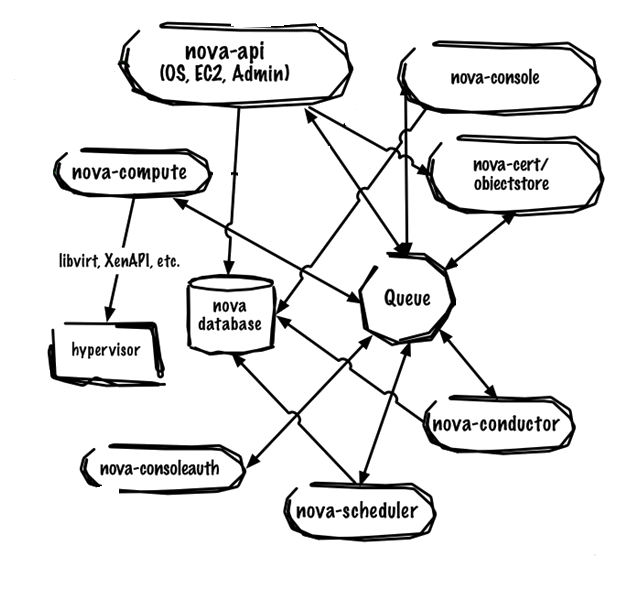
\includegraphics[clip= true, width= \columnwidth]{images/nova_components.png}
	\caption{OpenStack nova components and interactions}
	\label{fig:OSnovalogical}
\end{figure}
The two components of particular interest are the compute and the scheduler submodules.
The first submodule is a worker daemon called nova-compute, resides in each compute node and is in charge of creating and terminating virtual machine instances through hypervisor APIs, for example XenAPI for XenServer/XCP, VMwareAPI for VMware, libvirt for KVM and others as depicted in figure \ref{fig:OSnovacompute}.
Given that KVM and XenServer are popular choices for hypervisor technology and recommended for most use cases, OpenStack also wants to meet the needs of those administrators that don't have at their disposal a large computational power and might want to use a linux container technology such as LXC or Docker and wish to minimize virtualization overhead and achieve greater efficiency and performance. In addition to different hypervisors, OpenStack supports Intel as well as ARM and alternative hardware architectures.
The nova-compute agent is also in charge of letting the other nova submodules located in the controller node aware of its existence and status, this job is taken care of by sending periodical messages to the message broker service.
\begin{figure}[h]
	\centering
	% left bottom right top
	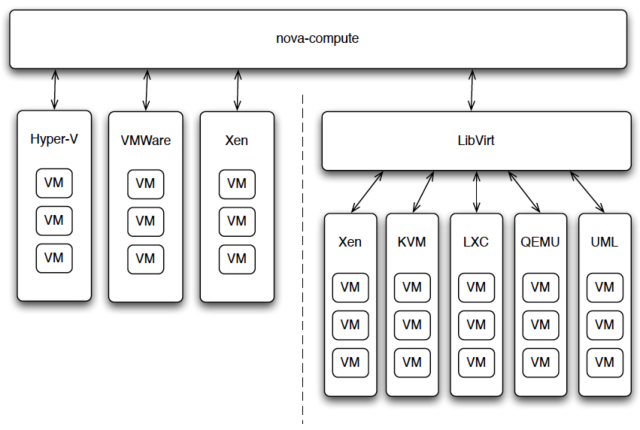
\includegraphics[clip= true, width= \columnwidth]{images/nova-compute.png}
	\caption{OpenStack nova components and communication}
	\label{fig:OSnovacompute}
\end{figure}
In the controller node are located both the module that manages requests (nova-api) and the nova-scheduler that is in charge of choosing where the virtual machines are going to be instantiated.
The scheduler submodule is highly important and valuable for an administrator that wants to maximize the efficiency of the entire system.
As default, OpenStack comes with an algorithm that takes decisions in a two-steps process called filter and weight, a representation of this sequence of events is given in figure \ref{fig:OSnovascheduler}.
In the first step, from all the available hosts are excluded the ones that don't meet specific requirements (e.g. free resources, architecture, hypervisor, etc) while in the second step all feasible hosts remained after the filtering are weighed according to a predefined cost function. The filter manager module is explicitly thought in a way that new constraints can be defined to further skim the pickable nova-compute module.
On the contrary of the filter module, the weighing function is customizable but unique so it has to be tuned with consciousness; its only purpose is to model each remaining host with a number, then the host with the highest value is chosen and the command to instantiate the virtual machine is dispatched to the corresponding nova-compute agent.
Both filter and weight take into consideration the information - generally referred as host status - exported by each nova-compute that typically consists in free resource availability.
\begin{figure}[H]
	\centering
	% left bottom right top
	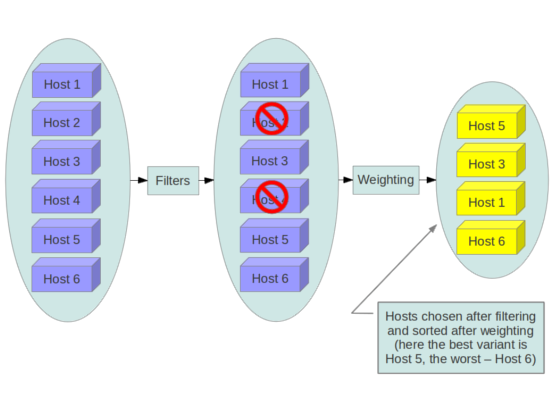
\includegraphics[clip= true, width= \columnwidth]{images/nova-filter-weight.png}
	\caption{OpenStack nova scheduler - filter and weight process}
	\label{fig:OSnovascheduler}
\end{figure}
\subsubsection{Network - neutron}
As well as nova, neutron is also a core component of OpenStack and is in charge of managing the network that interconnects the virtual machines.
Actually it would be more correct to say that it is in charge of managing the virtual overlay network that interconnects the virtual machines as it does not have any knowledge about the physical interconnections between compute nodes.
Neutron, formerly known as Quantum, provides users an abstraction that allow them to interconnect their own virtual machines and define some basic network services such as router, dynamic host configuration protocol (DHCP), firewall and virtual private network (VPN) terminator, decide which IP address assign to a VM and choose whether a VM is reachable from the Internet or not.
When a user decides to modify his/her own network topology or performs operations such as launching or stopping a virtual machine, neutron quickly reconfigures the vSwitches to provide connectivity and isolation.
In order to understand the level of abstraction provided by this component, is necessary to looks at the network at three different levels.
First comes the lower layer, composed by the physical equipments such as Ethernet cables, optical fibers and hardware switches, on top of this a full mesh of generic routing encapsulation (GRE) tunnels established between all the br-tun / br-net virtual switches infrastructure explained in section \ref{a:br_section}
Over this layer lays the actual user defined networks, modeled with virtual local area network (VLAN) and carries the traffic through the GRE tunnels.
This behavior is modifiable by intervening on the configuration files of neutron and therefore adapting this service to better suits the data-center communication infrastructure.
Being this flexible requires neutron to have a structure as the one in figure \ref{fig:neutron_structure} where five levels are indicated.
\begin{figure}[h]
	\centering
	% left bottom right top
	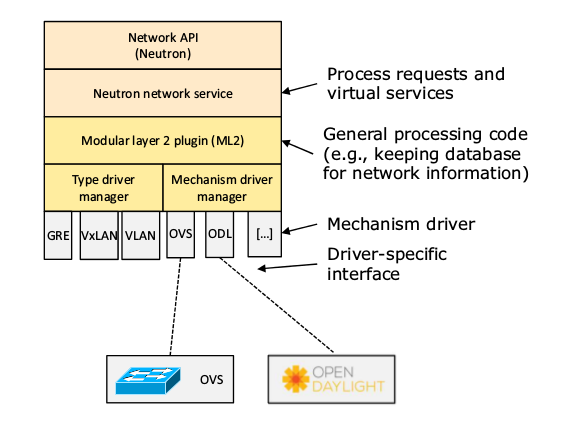
\includegraphics[clip= true, width= \columnwidth]{images/neutron_structure.png}
	\caption{OpenStack neutron - architecture}
	\label{fig:neutron_structure}
\end{figure}
The first two from the top are in charge of receiving requests, serialize and transform them into objects that models neutron resources.
The user is provided with a set of primitive to create its own network topology, offered resources are:
\begin{itemize}
\label{neutronresourcelist}
    \item Network - defines a L2 broadcast domain.
    \item Subnet - in a network, defines a IP address range
    \item Port - in a subnet, defines an attachment point for either a VM, a router or a firewall.
\end{itemize}
Scrolling down the architectural stack, there is the Modular Layer 2 plug-in (ML2) that is in charge of keeping the internal status of the network service to provide robustness and recoverability after a major failure of the neutron component. It also fulfill the "GET" requests that are useful for example to the dashboard to represent in a graphical manner all the information relative to the user's network topology.
Below the ML2 there are two managers layer that are in charge of dispatching requests to type and mechanism driver modules.
Both the driver kinds are intended to provide and implement per user and - if required - per user's network isolation, let's say that whether type drivers decides the standard that is going to be used, the mechanism is in charge of implementing it.
Type drivers are pluggable modules in which information about how to guarantee isolation are added to the neutron objects. The modified object is then returned to the third level of the stack that finally passes it to the other manager which is in charge of dispatching the received object to one or more drivers.
A mechanism driver is specifically designed to communicate with a particular virtual switch that resides in the compute nodes. This kind of component is crucial and each vendor can easily develop one that remaps neutron objects to commands specific to its device; OpenStack comes with already a lot of drivers from which to choose, for example the one for openvswitch, linuxbridge and the one developed expressly for the integration with OpenDaylight which will be described in section \ref{sec:opendaylight}.
Mechanism drivers are actually called two times each time a resource is created, updated or deleted, once before the ML2 database operation and then called again once the data-base transaction is concluded successfully.
This double call is intended so that before the ML2 commit the mechanism driver prepares and checks the feasibility of the operation and once it receives the grant from the upper layer, the operation is actually performed.
To summarize, this service other than providing connectivity between VMs, also does the opposite, establishing user isolation in a way that inter-user communication can happen only via a public network defined by the administrator and meant for this specific purpose.

\subsubsection{Orchestration - heat}
Heat is the main project in the OpenStack Orchestration program. It implements an engine to launch multiple composite cloud applications based on templates in the form of text files that can be treated like code. It aims to export a unique-common API usable by the user to instantiate a complete network topology comprehensive of virtual machines in the form of a template making just one call; the Heat engine then takes care of translating such template into calls for both nova and neutron. In order to improve performances, all these calls will be made in parallel unless dependencies between resources are implicitly or explicitly specified. As an example of implicit dependency let's consider neutron resources listed in \ref{neutronresourcelist}.
A neutron port attached to a network can exist only if that specific network has already been created.
On the other hand, as explicit dependence the user can point out that a virtual machine must be created before another one - a valid motif can be that the first VM provides services without those the second one cannot boot correctly.
Another useful feature is the management of updates.
When a request is received by Heat and results to contain a reference to an already instantiated template, the engine is able to understand what is changed between the allocated resources and the ones present in the request - this is done similarly to the "diff" unix/linux command.
Once this task has come to an end, the creation, modification and/or deletion of resources will be handled; the new will be created and the no more needed can be deleted.
For what concerns the update of a resource, Heat allows two ways of behavior. The first one is to rawly destroy the elder and then create a new one with the up-to-date characteristics. A more sophisticated approach is to define in each service the way to handle the update locally (e.g. change the static ip address of a port), however this is not always possible - as an example in the case of changing the disk image of a VM.

\subsubsection{Dashboard - horizon}
Usability is essential in complex systems so programmers typically offers a user friendly interface, avoiding the unexperienced users the pain of going through a complex command line tool.
Under this aspect OpenStack is no exception and provides a well structured web dashboard called Horizon from which administrators can monitor the system and users can easily perform operations that otherwise require a long list of command-line inputs.
The dashboard follows the OpenStack's main concept of abstraction and models VMs, networks and network services in a way that even an unexperienced user can easily understand, in figure \ref{fig:OSdashboard} is given a screen-shot of what a user sees when a simple topology is deployed. As is evident from the image, there is no indication about the physical location of the VMs (VM1, VM2, VM3) or the service (Router) nor about other user instances.
\begin{figure}[h]
	\centering
	% left bottom right top
	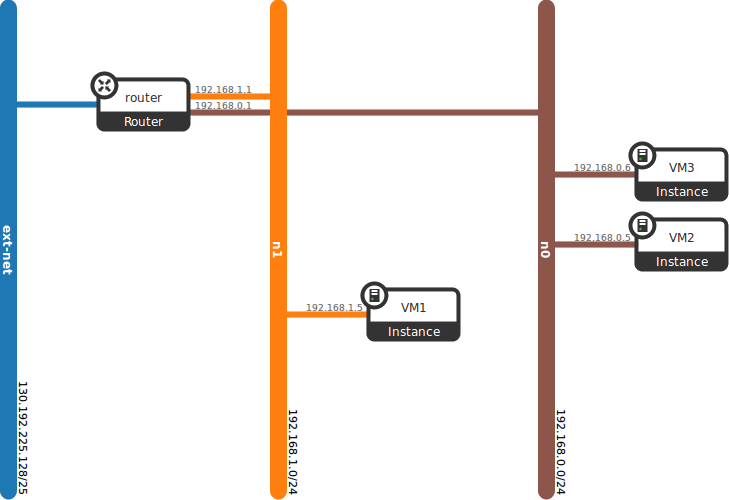
\includegraphics[clip= true, width= \columnwidth]{images/neutron-topology-example.png}
	\caption{OpenStack dashboard - example of network topology design with VMs}
	\label{fig:OSdashboard}
\end{figure}

\subsubsection{Command line clients}
Since all services are meant to receive commands via REST API, OpenStack developers have produced a command-line based client for each project that automates otherwise pedantic operation and complex typing of unicode strings.
These clients perform a series of cURL requests to obtain the required result.
As an example lets say that a user wants a list of all his/hers virtual machines with some details, using the client it comes easy in fact is necessary to type "nova list"; to achieve the very same result, it is mandatory to acquire an authentication token, then use it to query the nova-api and obtain the list of instances. If more details are required, a request for each machine has to be dispatched.
Other than automation, clients provide also data presentation so instead of receiving responses in form of raw json or xml, better-looking and compact tables are displayed.

\section{OpenDaylight}
\label{sec:opendaylight}
OpenDaylight (ODL), as presented in the official project website\cite{Opendaylightwebsite}, is an open platform for network programmability to enable SDN and NFV for networks.
The software is a combination of components including a fully pluggable controller, interfaces, protocol plug-ins and applications. With this common platform both customers and vendors can innovate and collaborate in order to commercialize SDN and NFV based solutions.
If stripped to its very minimal core, it results to be just an openflow controller, which is able to instruct the controlled switches to behave in a certain way.
There are numerous openflow controller projects since the standard came out back in December 2009 but there are factors that really differs OpenDaylight from the others; first there is the community that keeps developing it, some major vendors such as Cisco, IBM, HP, Brocade Juniper, Microsoft and others also support the project both economically and with workforce.
Secondly it has been engineered to make easy for developers to add their additions in form of a bundle that will easily integrate and interact with the core components and other plug-ins either available in the public repository, proprietary or created by other developers.

\section{Integration between the two projects}
Already in the first official stable release of OpenDaylight - codename Hydrogen - published in February 2014 and in particular in the "virtualization" version, a plug-in for the integration with OpenStack was made available. This add-on represent the first step towards what will likely become the de facto standard for data-centers management. Being in its early times, the OpenDaylight framework and therefore the functionalities exported to OpenStack Neutron, the behavior is sometimes different from the expected one; either way making this two software products work together in a cooperative way is an aspect of particular interest. In fact as mentioned before OpenStack sees the entire underlaying physical network as a commodity and has no control over it, OpenDaylight on the other hand has been projected to do exactly so.
The integration between the two projects will result with the possibility to aggregate the full control of the data-center in the aspects of both managing the compute and tuning the network accordingly in an automated and robust way with lot of space for improvement and optimization of performances and capabilities resulting in a better quality of service (QoS), lower management cost and even in the chance of offering users new custom functionalities.
However leveraging these functionalities requires an OpenDaylight fully controlled network and in order to allow that the whole data-center communication system needs to be openflow-capable.
Given that openflow physical switches are still not so common on the market, having the possibility to pilot them with the very same controller that manages the virtual switches in the compute nodes will be an enormous plus for the data-center network administrators whom will be allowed to control, configure and monitor all the devices from a unique and centralized point.


%This is a reference to a chapter \ref{chap:quo}. This is a reference to a figure \ref{fig:doge}. This is a reference to some code \ref{lst:hello}. This is a citation \cite{famous:paper}.
%
%\lstinputlisting[label=lst:hello, firstline=2, lastline=4, caption={I directly included a portion of a file}]{code/hello.py}
%
%\begin{lstlisting}[language=Java, label=lst:java, caption={Some code in another language than the default one}]
%public void prepare(AClass foo) {
%        AnotherClass bar = new AnotherClass(foo)
%}
%\end{lstlisting}
%
%\Blindtext
%
%\begin{figure}
%\begin{center}
%\includegraphics[width=0.5\columnwidth]{images/doge.png}
%\end{center}
%\caption{This is not a figure. It's a caption.}
%\label{fig:doge}
%\end{figure}